\documentclass[runningheads,a4paper]{llncs}
\usepackage{amssymb}
\setcounter{tocdepth}{3}
\usepackage{listings}
\usepackage{booktabs}
\usepackage{mathtools}
\usepackage{tabularx}
\usepackage{fixltx2e}
\PassOptionsToPackage{hyphens}{url}\usepackage{hyperref}
\usepackage[hyphens]{url}
\usepackage{upquote,textcomp}
\lstset{breaklines=true, basicstyle=\scriptsize\ttfamily, upquote=true}

\usepackage{fancyvrb}
\VerbatimFootnotes
\usepackage{cprotect}

\usepackage{graphicx}
\makeatletter
\def\maxwidth#1{\ifdim\Gin@nat@width>#1 #1\else\Gin@nat@width\fi}
\makeatother

\usepackage{amsmath}
\usepackage{pmml-new}

\usepackage{color,graphics,array,csscolor}

\usepackage{fontspec,unicode-math}
\usepackage[Latin,Greek]{ucharclasses}
\setTransitionsForGreek{\fontspec{Times New Roman}}{}

\usepackage{subscript}
\lstset{breaklines=true, basicstyle=\scriptsize\ttfamily}

\begin{document}
\mainmatter

\title{euBusinessGraph: Company and Economic Data for Innovative Products and Services}
\titlerunning{euBusinessGraph}
\author{Vladimir Alexiev\inst{1} \and
Atanas Kiryakov\inst{1} \and
Plamen Tarkalanov\inst{1}}
\authorrunning{Vladimir Alexiev et al.}
\institute{Ontotext Corp\\
\email{vladimir.alexiev@ontotext.com, 
atanas.kiryakov@ontotext.com, 
plamen.tarkalanov@ontotext.com}}
\maketitle

\begin{abstract}
Corporate information, including basic company firmographics (e.g., name(s), incorporation data, registered addresses, ownership and related entities), financials (e.g., balance sheets, ratings) and contextual data (e.g., addresses, economic activity classification, key officers, public tenders data, press mentions and events) are the foundation that many data value chains are built on. Furthermore, this type of information contributes to the transparency and accountability of enterprises, is instrumental when input to the process of marketing and sales, and plays a key role in many business interactions. Collecting and aggregating data about a business entity from several public sources (be it private/public, official or non-official ones), and especially across country borders and languages is a tedious, time consuming, error prone, and expensive operation which renders many potential business models non-feasible.

The euBusinessGraph project integrates European company and economic data from various data providers, including OpenCorporates (the largest open database of company info crawled from official registers), Norway's Bronnoysund Register Center (official register data), SpazioDati (rich IT data from official registers, additional databases, web crawl of company sites, tender info, etc.), EventRegistry events, GLEI, Panama Leaks, etc.

euBusinessGraph is intended to overcome these barriers and provision several important business cases, such as economic journalism (Deutsche Welle), publication of rich company data (BRC), tender information service (CERVED), business intelligence (EVRY), etc. It will also provide a marketplace of company data, with some free search and faceting, leading to information about richer Data Offerings by specific providers and their pricing.

We will present the work done on exploring relevant ontologies and vocabularies for describing companies, systems of identifiers, development of a unified data model, plans for data flows, data aggregation, matching and cross-linking, and the opportunities that lie ahead for the business cases and the data marketplace.

This session will demonstrate services like company popularity ranking, monitoring mentions of related entities in news and finding suspicious relation patterns in FactForge -- a knowledge graph with more than 2 billion edges of POL (persons, organizations, locations) data interlinked with 1 million news articles. 

An accompanying poster\footnote{\url{https://github.com/VladimirAlexiev/VladimirAlexiev.github.io/raw/master/pubs/euBusinessGraph-poster-Semantics2017.pdf}} and presentation are available.

\keywords{business graph, company data, economics, euBusinessGraph, firmographics, linked data, public procurement}
\end{abstract}


\section{Introduction}

euBusinessGraph is a 30-month research project funded by the EU H2020 programme on Big Data integration and experimentation that started in January 2017. Its purpose is to integrate a large number of economics-related datasets such as companies, public procurement tenders, company events, etc.; to provision 6 business cases using that data; and to establish a data marketplace for such data. The project partners comprise:
\begin{enumerate}
\item SINTEF\footnote{\url{https://www.sintef.no/en/}}, Norway's largest research organization;
\item OpenCorporates\footnote{\url{https://opencorporates.com/}}, the largest aggregation of company data from official registers;
\item Cerved\footnote{\url{https://www.cerved.com/}}, an Italian leader in business information;
\item SpazioDati\footnote{\url{http://www.spaziodati.eu/}}, an innovative provider of data about Italian companies (Atoka\footnote{\url{http://atoka.io/}});
\item EVRY\footnote{\url{https://www.evry.com/en/}}, Norway's largest IT services provider;
\item Deutsche Welle\footnote{\url{http://www.dw.com/}} (DW), Germany's international broadcaster;
\item Ontotext\footnote{\url{https://ontotext.com/}}, a world leader in semantic technologies, databases and semantic cloud offerings;
\item Brønnøysund Register Centre\footnote{\url{https://www.brreg.no/home/}} (BRC), Norway's national business register agency (18 registers);
\item Institut "Jozef Stefan"\footnote{\url{https://www.ijs.si/}} (IJS), creator of EventRegistry\footnote{\url{http://eventregistry.org/}} (6.5M world events extracted from 190M articles);
\item University of Milano-Bicocca\footnote{\url{http://www.unimib.i/}} (UNIMIB), specializing in data management and service science.
\end{enumerate}

The project concept including data value chain and customer segmentation, is shown below.
\begin{figure}[h!]
\centering
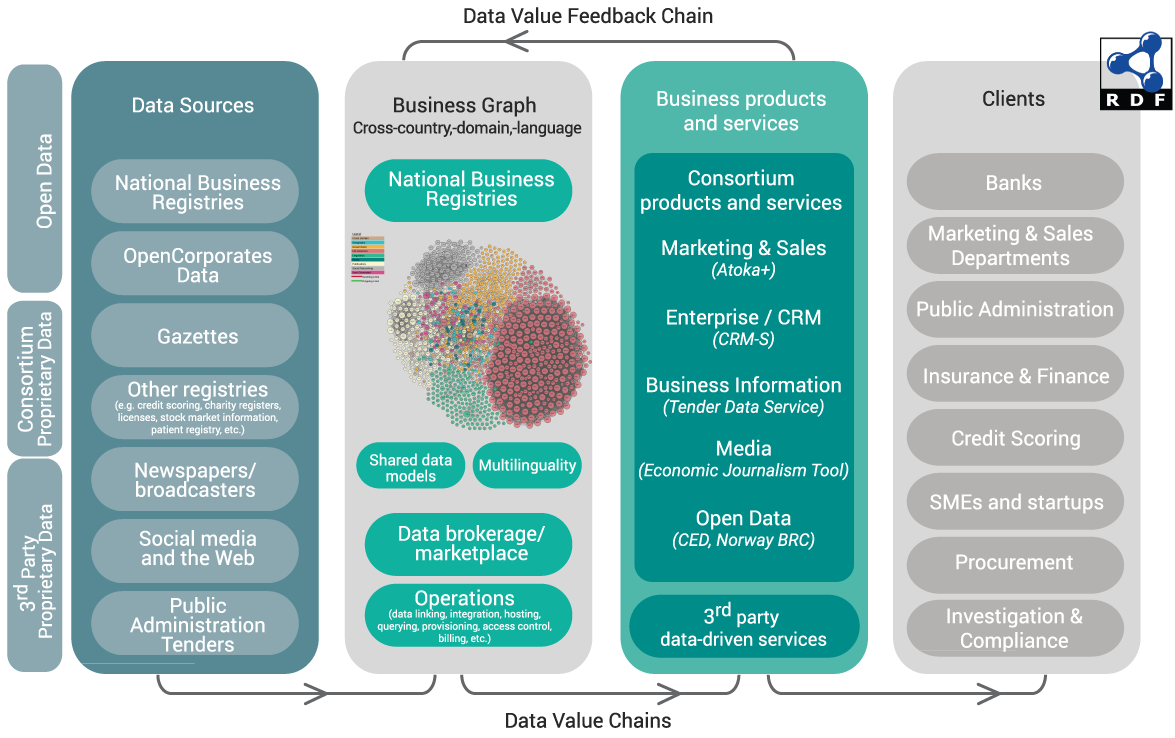
\includegraphics[width=\maxwidth{\textwidth}]{img/1000020100000497000002E2C8E24D0717D0E9B2.png}
\cprotect\caption{Project Concept}
\label{}
\end{figure}


\section{Business Cases and Lean Business Modeling}

The business cases addressed by the project include the following:
\begin{itemize}
\item OpenCorporates will enlarge its offering with a Corporate Events Data Service. It will increase the number of EU Government Gazettes ingested (see OpenGazettes\footnote{\url{http://opengazettes.com/}}) and add non-register sources of company events.
\item Cerved will implement a Tender Discovery Service that will integrate data from various sources of public procurement info and implement a recommendation component that can suggest relevant tenders to companies.
\item SpazioDati will increase the reach of its Atoka\footnote{\url{http://atoka.io/}} company information service (Atoka+) by aggregating data about more countries.
\item Deutsche Welle will implement a new Economic Journalism tool to save cost in the editorial department and increase public reach through improved story telling.
\item EVRY will leverage the business graph to be developed by the project in a set of Customer Relationship Management (CRM) systems, increasing data reach and quality.
\item BRC will publish the full spectrum of official register data in RDF and describe the data in a semantic way, increasing the value of Norwegian LOD.
\end{itemize}

Business case development proceeds in an agile fashion, using Lean Business Modeling and Minimum Viable Product approaches to ensure the developed products meet market demand. We use tools such as Product Vision Statement, Lean Business Model Canvas, Value Proposition Canvas, GO product roadmap, Test card, and Learning card as adopted by SINTEF's innovation department. Below is an example of a lean Business Model Canvas  \cite{_Ref491191527} for Atoka+
\begin{figure}[h!]
\centering
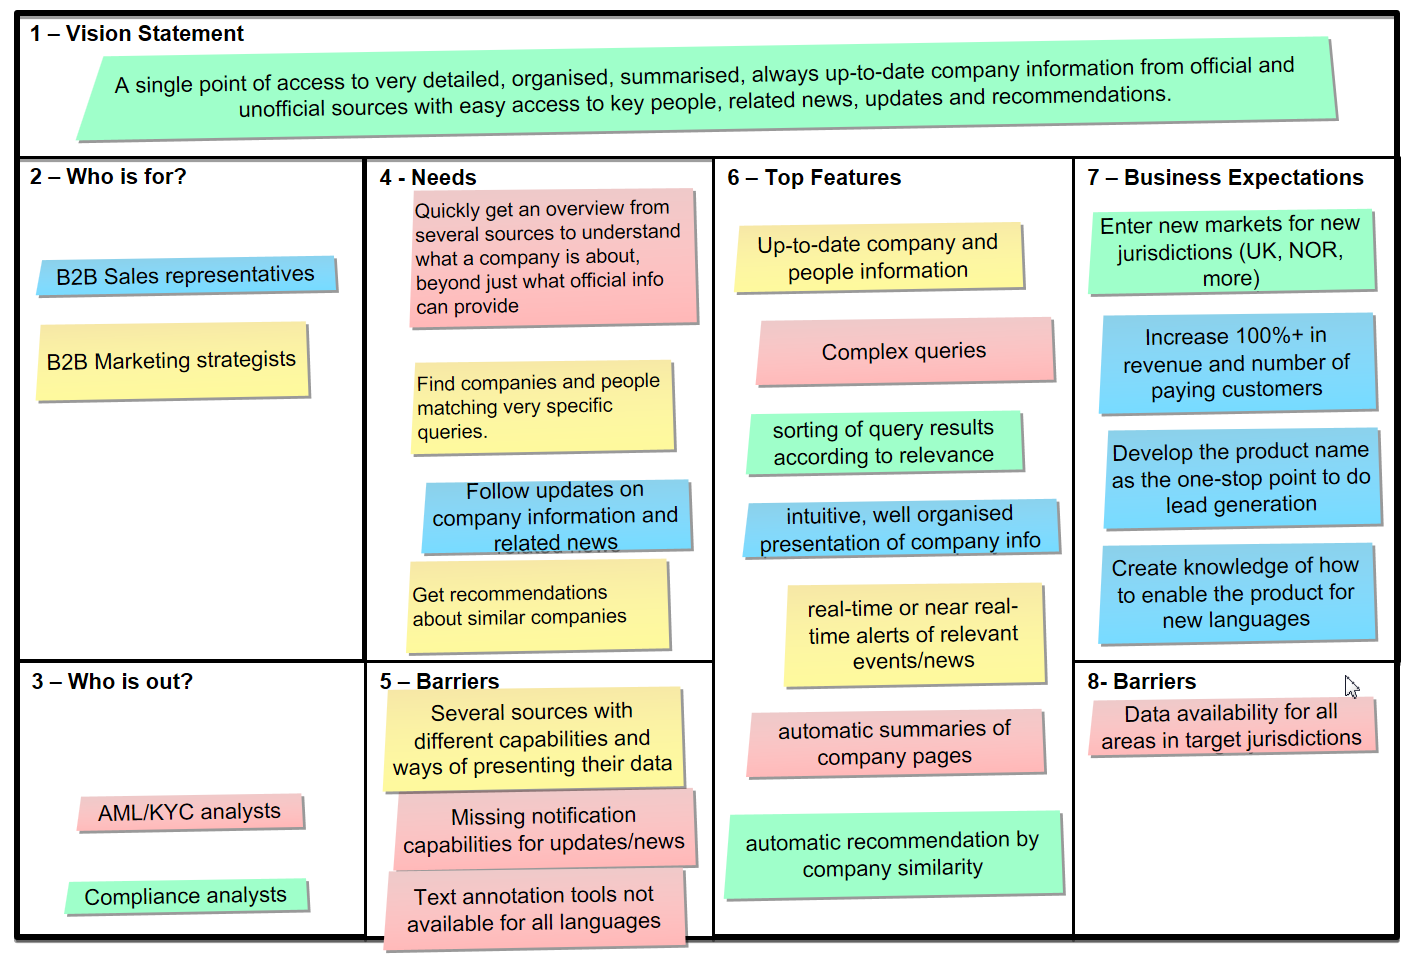
\includegraphics[width=\maxwidth{\textwidth}]{img/1000020100000587000003BFCD6E24D0654D050D.png}
\cprotect\caption{Example Business Model Canvas}
\label{}
\end{figure}


Various monetization models are considered by the partners, including free, freemium and paid (for premium data). Describing such dataset offerings is an important function of the project.
\begin{figure}[h!]
\centering
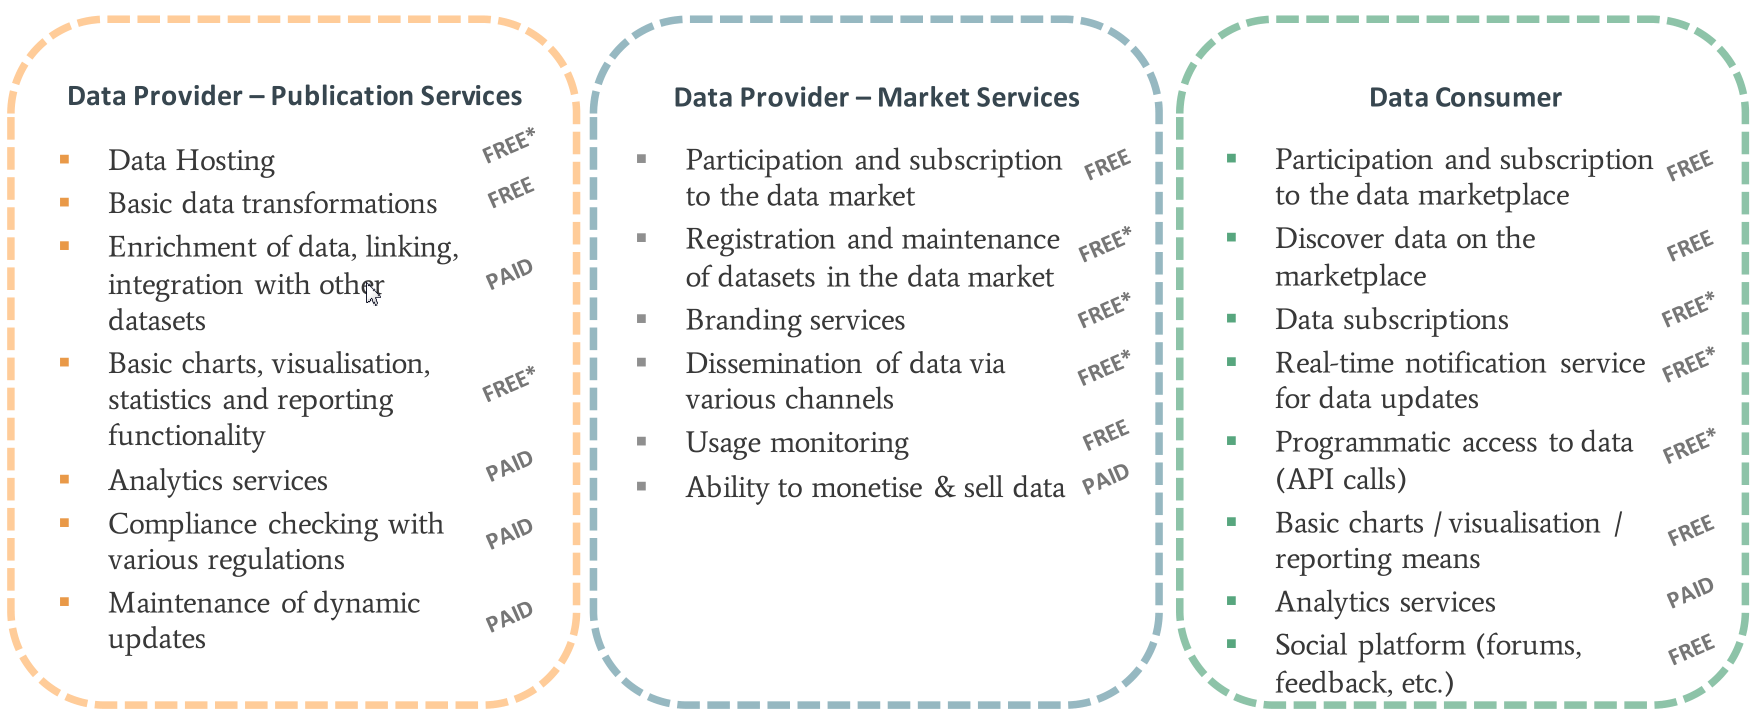
\includegraphics[width=\maxwidth{\textwidth}]{img/10000000000006E1000002CB881B70F373419303.png}
\cprotect\caption{Example Monetization Models}
\label{}
\end{figure}


\section{Company Datasets and Ontologies}

The project studied numerous ontologies and datasets that represent company and related economic data, and which were taken into account when creating the project's data model. Amongst them are:
\begin{enumerate}
\item Global Legal Entity Identifier (GLEI)  \cite{_Ref491193712};
\item Business Registers Interconnection System (BRIS)  \cite{_Ref491193639} \cite{_Ref491194142};
\item Financial Industry Business Ontology (FIBO)  \cite{_Ref491193410};
\item OpenCorporates schema  \cite{_Ref491194336};
\item Bulgarian Trade Register schema  \cite{_Ref491193979};
\item W3C Organization ontology  \cite{_Ref491194417};
\item W3C Registered Organization ontology  \cite{__RefNumPara__857_1597909725};
\item W3C Location ontology  \cite{_Ref491194659};
\item Dun \& Bradstreet company data;
\item Panama Papers offshore company dataset  \cite{_Ref491193106} and its RDF representation Linked Leaks  \cite{_Ref491193118};
\item Wikidata properties for describing companies, especially company identifiers in various registers;
\item A number of related and subsidiary ontologies and code lists such as Schema.org, Dublin Core, IANA language tags, NUTS and LAU (EU administrative regions), NACE (EU economic activities), etc.
\end{enumerate}

 \cite{_Ref491191838} presents some of these data artefacts, and relates each of them to the "5V" of big data (Variety, Volume, Velocity, Veracity, leading up to Value). Many of these data sources are not in semantic format, therefore mapping and conversions are required if they are to be integrated semantically. Below is an example of such mapping: the GLEI XML schema to the FIBO ontology and a custom GLEI Ontology (GLEIO)  \cite{_Ref491193086}.
\begin{figure}[h!]
\centering
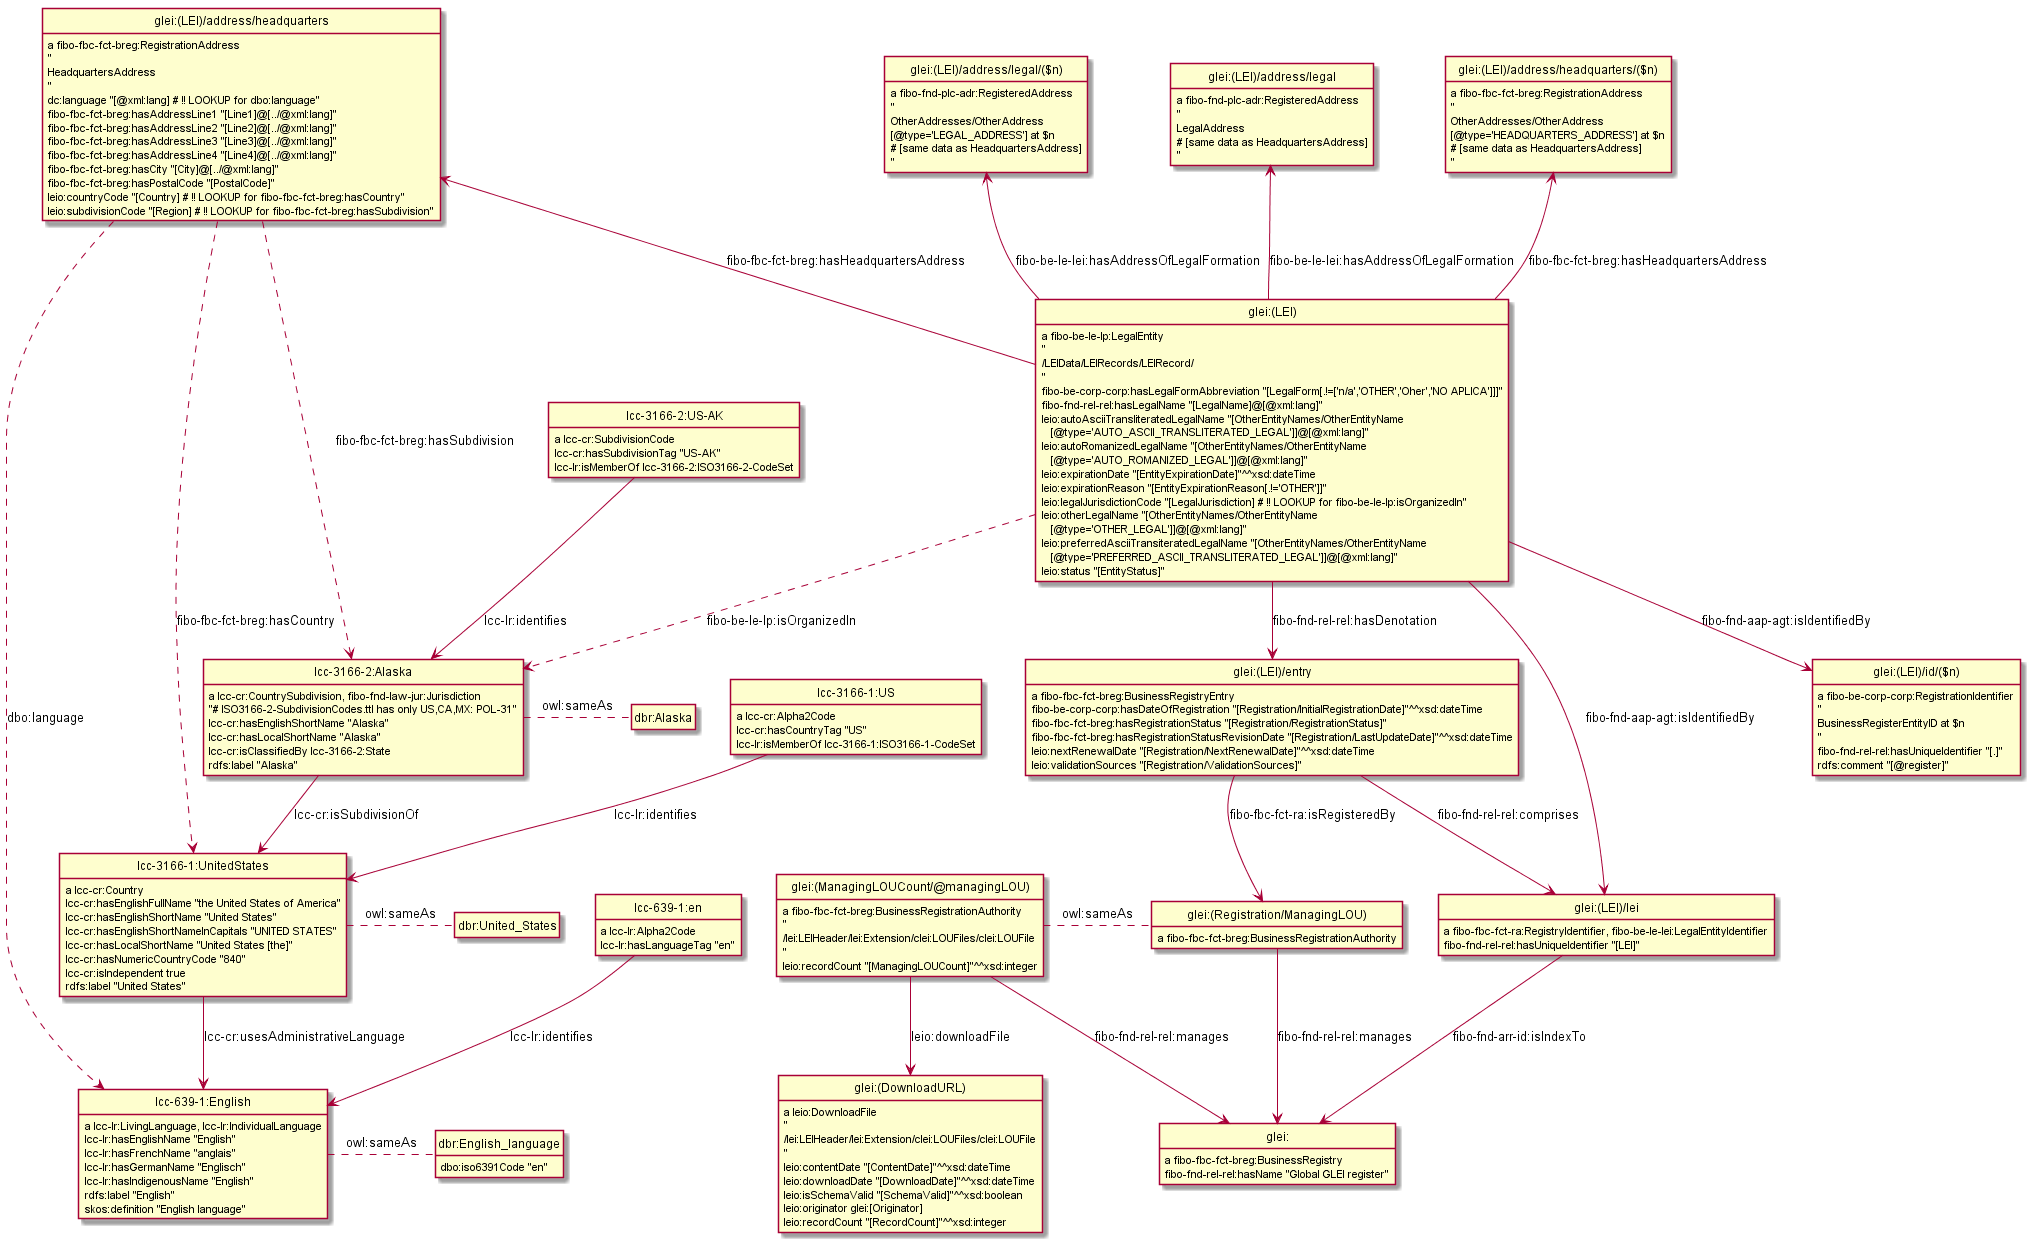
\includegraphics[width=\maxwidth{\textwidth}]{img/10000000000007EF000004DB2899AFE905260A79.png}
\cprotect\caption{Mapping of GLEI to FIBO and GLEIO}
\label{}
\end{figure}


\section{Semantic Data Model}

The euBusinessGraph semantic data model  \cite{_Ref491194758} is a synthesis of the various data artefacts that we studied, fulfilling the data needs of the project. It includes detailed treatment of classes, properties, values, scope notes, data provider rules, URL conventions, etc. It reuses ontologies such as W3C Org, RegOrg, Locn, ADMS; DC, DCT, schema.org, SKOS, SIOC. It reuses datasets such as NACE (economic classification), NUTS+LAU (EU regions), GLEI RAL (registration authority list). 

This initial draft covers companies, company types, status, addresses, NUTS+LAU regions, NACE classification of economic activity and registrations (identifiers). We will shortly add detailed information about registers: dataset offerings, what level of detail they cover, per-company URL templates, MIME types. Future versions will add information about officers (directors, executives), provenance (who contributed which data). We used rdfpuml  \cite{_Ref491433543} to generate semantic model diagrams (see Fig.~\ref{refFigure4}) and Object-Role Modeling through the Norma tool  \cite{_Ref491195242} (see Fig.~\ref{refFigure5}) to generate an RDF representation.
\begin{figure}[h!]
\centering
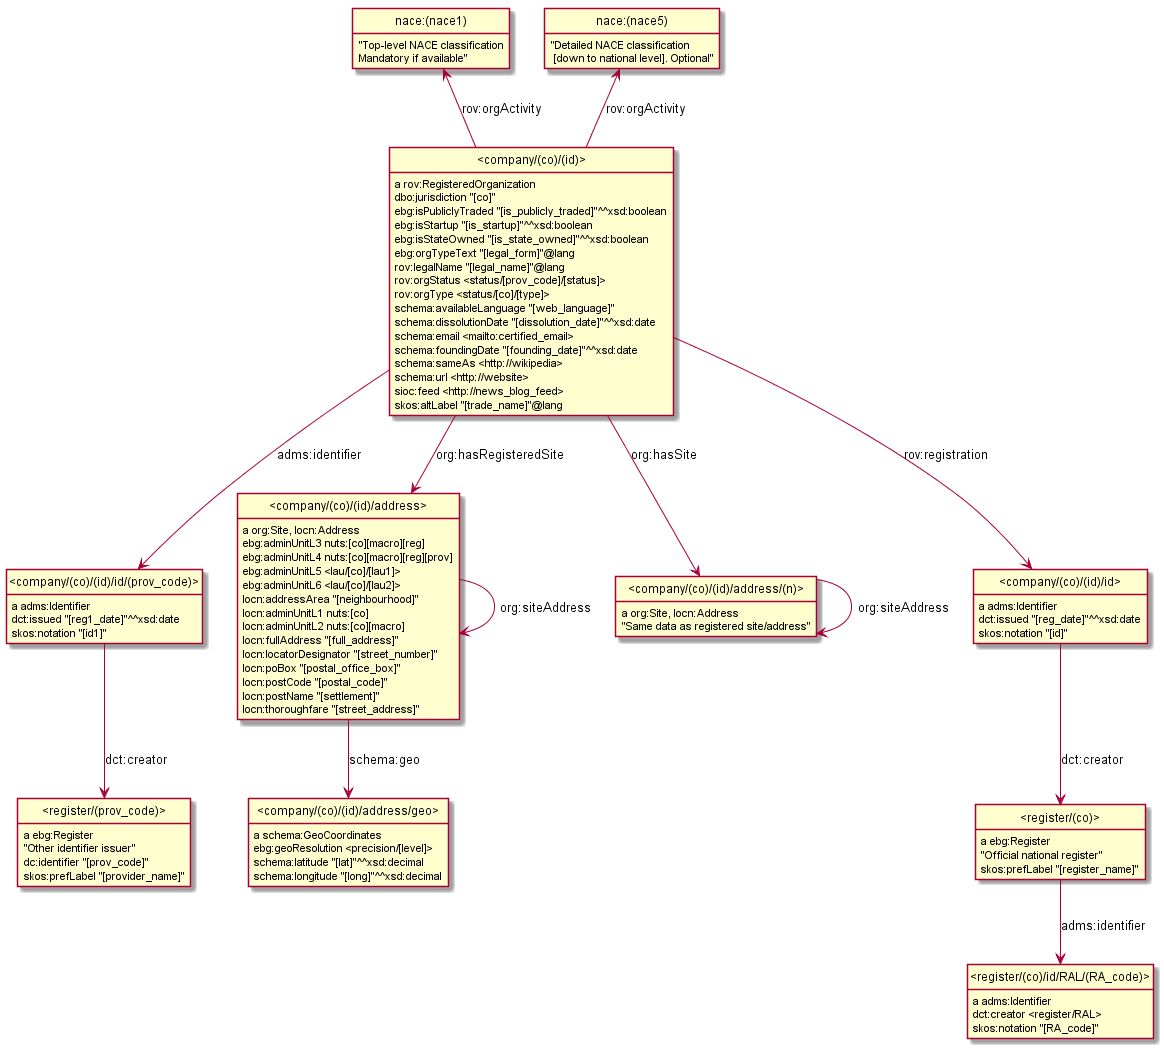
\includegraphics[width=\maxwidth{\textwidth}]{img/100000000000048C00000419A8A0F6AE07037D76.png}
\cprotect\caption{euBusiness Graph Semantic Model Diagram}
\label{refFigure4}
\end{figure}



\begin{figure}[h!]
\centering
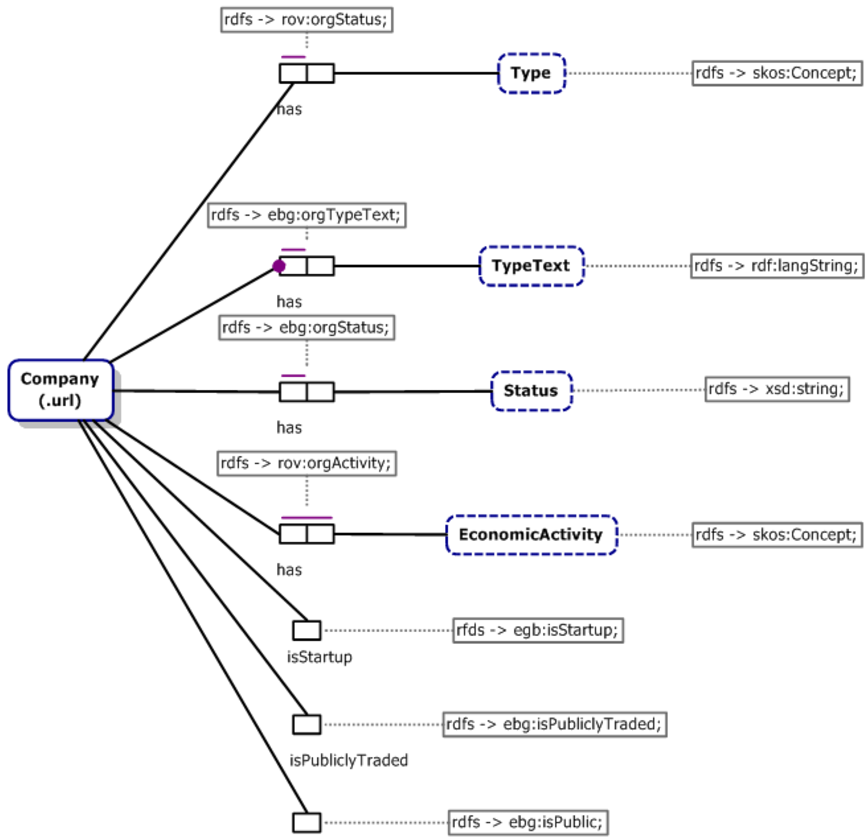
\includegraphics[width=\maxwidth{\textwidth}]{img/100000000000036300000348EF8D1F5319A59BDD.png}
\cprotect\caption{Object-Role Diagram of Part of the Semantic Model}
\label{refFigure5}
\end{figure}


\section{Technologies Used}

In addition to partner datasets, the project may use some of the following technologies and tools:
\begin{enumerate}
\item The Ontotext GraphDB\footnote{\url{http://graphdb.ontotext.com/}} (formerly OWLIM) semantic database  \cite{_Ref491415452}
\item Ontotext Cognitive Cloud\footnote{\url{https://ontotext.com/products/cognitive-cloud/}} (successor of the Self-service semantic system\footnote{\url{http://s4.ontotext.com/}}) provides on-demand access to text analytics, semantic graph databases and Linked Data technology in the cloud (Amazon Web Services). A user can start building Smart Data prototypes without the need for licensing, provisioning, installation and maintenance. In the project, the Cognitive Cloud will be used as platform for developing, running and hosting the euBusinessGraph Marketplace and Services. 
\end{enumerate}
\begin{figure}[h!]
\centering
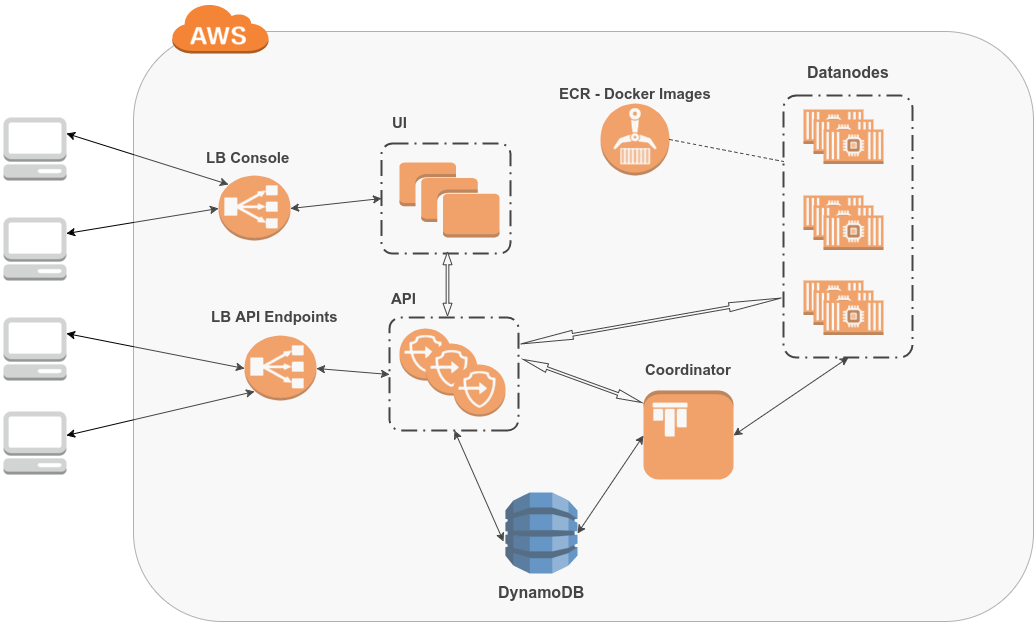
\includegraphics[width=\maxwidth{\textwidth}]{img/100002010000040A0000026E32942332B6CAF0DA.png}
\cprotect\caption{Ontotext Cognitive Cloud Architecture}
\label{}
\end{figure}

\begin{enumerate}
\item DataGraft\footnote{\url{https://datagraft.net/}} \cite{__RefNumPara__7260_1562275339} \cite{_Ref491437414} "One stop shop for hosted data management" is a tool to interactively build, modify and share data transformations; reuse transformations to repeatably clean and transform spreadsheet data; and finally host and share datasets in a semantic way. 
\item RDF by Example  \cite{_Ref491433543} is an Ontotext tool for semantic modeling and R2RML Generation
\item Dandelion \footnote{\url{https://dandelion.eu/}}API\footnote{\url{https://dandelion.eu/}} is a semantic text analysis tool used by SpazioDati.
\item Wikifier\footnote{\url{http://wikifier.org/}} is a semantic annotation tool for 100s of languages used by JSI for EventRegistry.
\item ABSTAT\footnote{\url{http://abstat.disco.unimib.it/}} is a tool for Linked Data Summarization with ABstraction and STATistics by UNIMIB.
\end{enumerate}

Other semantic conversion tools that may potentially be used include:
\begin{enumerate}
\item TARQL\footnote{\url{https://tarql.github.io/}} is a command-line tool for converting CSV files to RDF using SPARQL 1.1 syntax.
\item XSPARQL\footnote{\url{http://xsparql.deri.org/}} \cite{__RefNumPara__8272_1562275339} is W3C submission\footnote{\url{http://xsparql.deri.org/spec.html}} for a query language that melds XQuery  \cite{__RefNumPara__7336_1562275339} and SPARQL  \cite{__RefNumPara__859_1597909725}, and the respective tool that implements it. It transforms XML, JSON and relational data (RDB2RDF) to RDF (lifting), SPARQL querying and conversions to other formats (lowering), the full power of XQuery for control flow and sequence processing, and scripting for Web data integration in general.
\end{enumerate}

\section{Demonstration with FactForge}

As part of our presentation, we demonstrate services such as company popularity ranking, monitoring mentions of related entities in news, and finding suspicious relation patterns. We use data from FactForge\footnote{\url{http://factforge.net/}} \cite{__RefNumPara__3722_1458423281}, a knowledge graph of about 2 billion triples. It represents a hub of open data and news about persons, organizations and locations (POL data):
\begin{enumerate}
\item Popular LOD datasets: DBPedia, Geonames, WorldFacts and Wordnet.
\item POL data: Panama Papers, GLEI, Trump World. People and organizations from these datasets are mapped to DBPedia. The schemata of these datasets and DBPedia are partially mapped to FIBO classes and relationships in order to allow for unified querying and analytics across the different datasets.
\item A live stream of news metadata, linking the articles to entities and concepts: about 2000 news per day tagged with the N\footnote{\url{http://now.ontotext.com/}}ews \footnote{\url{http://now.ontotext.com/}}O\footnote{\url{http://now.ontotext.com/}}n the \footnote{\url{http://now.ontotext.com/}}W\footnote{\url{http://now.ontotext.com/}}eb (NOW) semantic news demonstrator.
\end{enumerate}

FactForge allows one to play with the data through GraphDB's Visual Graph Explorer -- a customizable interactive exploration tool (see below). See  \cite{_Ref491439427} for a detailed report on visualization capabilities.
\begin{figure}[h!]
\centering
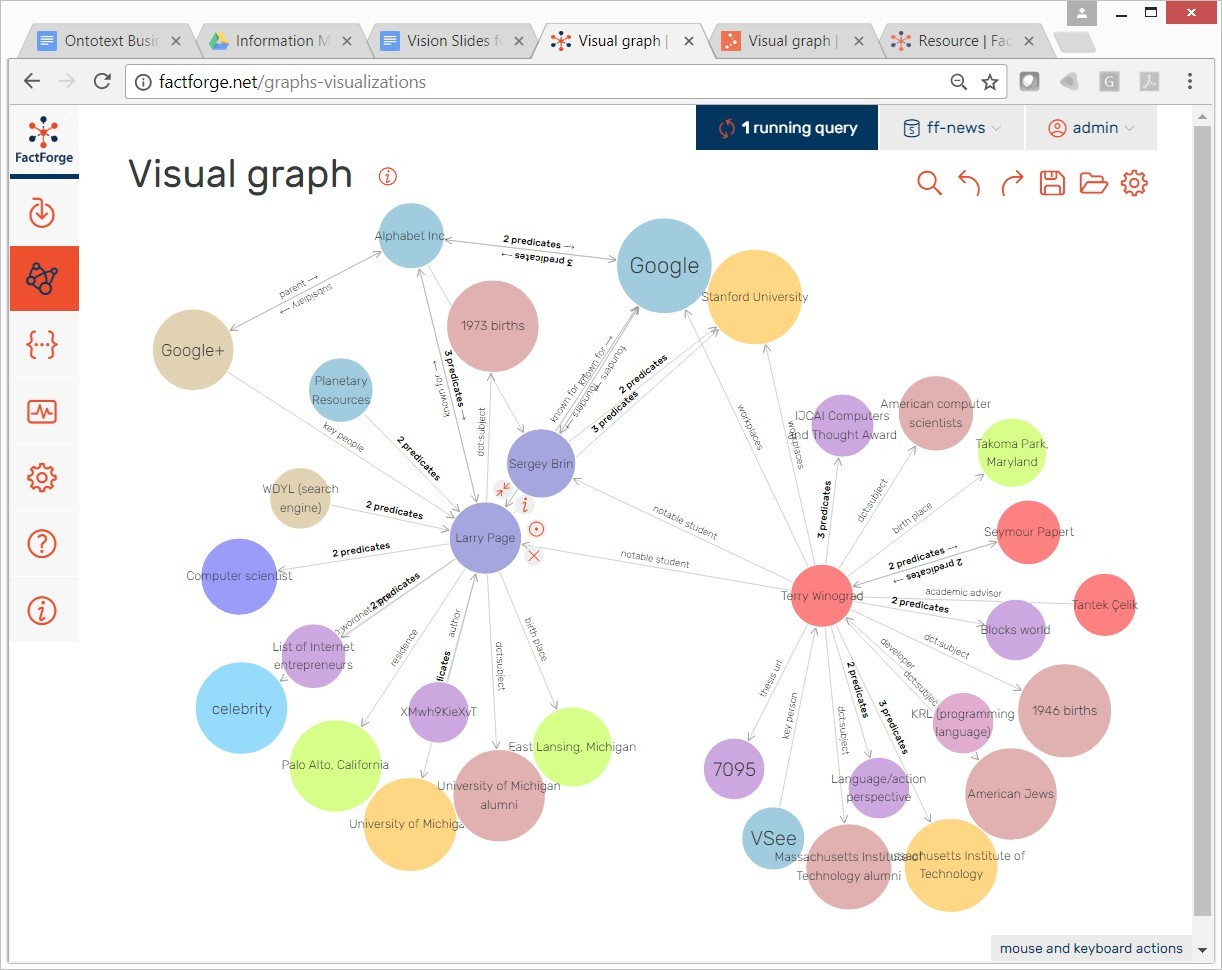
\includegraphics[width=\maxwidth{\textwidth}]{img/10000000000004C6000003CA6EE0A0766E99B97E.jpg}
\cprotect\caption{GraphDB Workbench Visual Graph}
\label{}
\end{figure}


Sample queries in FactForge demonstrate media monitoring, tracing company control, industry trends and statistics. One of them is a SPARQL query that detects the following pattern: a company that controls another company in the same country, through a company registered in an offshore zone.

Finally, Rank\footnote{\url{http://rank.ontotext.com/}} is a demonstration service for news popularity ranking of companies. It supports ranking with consolidation of mentions of subsidiaries and is based on FactForge.
\begin{figure}[h!]
\centering
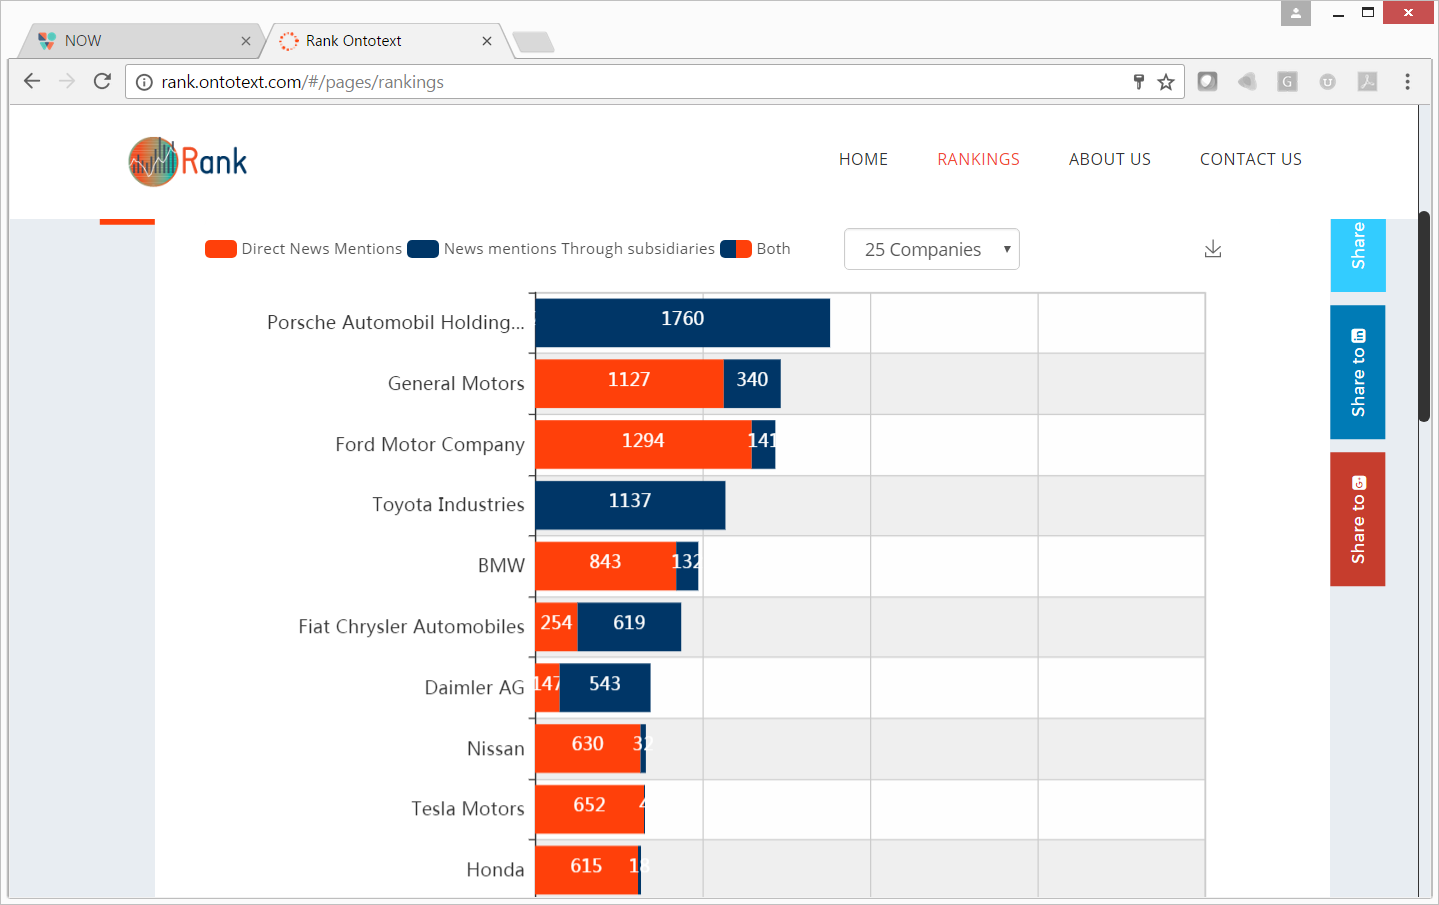
\includegraphics[width=\maxwidth{\textwidth}]{img/100000000000059F00000389BBBF66F35F310098.png}
\cprotect\caption{Global Ranking of Automotive Companies}
\label{}
\end{figure}


\subsubsection*{Acknowledgements.}euBusinessGraph has received funding from the EU H2020 research and innovation programme "Big Data PPP: cross-sectorial and cross-lingual data integration and experimentation" under grant agreement No 732003.


\begin{thebibliography}{4}

\bibitem{_Ref491191527} Alexander Osterwalder, Yves Pigneur. Business Model Generation\footnote{\url{https://strategyzer.com/books/business-model-generation}}, 2010.
\bibitem{_Ref491194659} Andrea Perego, Michael Lutz. ISA Programme Location Core Vocabulary\footnote{\url{https://www.w3.org/ns/locn}}. Second version, 2015-03-23
\bibitem{_Ref491415452} Barry Bishop, Atanas Kiryakov, Damyan Ognyanoff, Ivan Peikov, Zdravko Tashev, Ruslan Velkov. OWLIM: A Family of Scalable Semantic Repositories.\footnote{\url{http://www.semantic-web-journal.net/sites/default/files/swj97_1.pdf}} Semantic Web Journal, Volume 2, Number 1. May 2011.
\bibitem{__RefNumPara__8272_1562275339} Daniele Dell'Aglio, Axel Polleres, Nuno Lopes, and Stefan Bischof. Querying the Web of Data with XSPARQL 1.1\footnote{\url{http://ceur-ws.org/Vol-1268/paper19.pdf}}. ISWC Developers Workshop, 2014
\bibitem{_Ref491194417} Dave Reynolds. The Organization Ontology\footnote{\url{http://www.w3.org/TR/vocab-org/}}, W3C Recommendation, 16 January 2014
\bibitem{__RefNumPara__7260_1562275339} Dumitru Roman, Marin Dimitrov, Nikolay Nikolov, Antoine Putlier, Brian Elvesæter, Alex Simov, Yavor Petkov. DataGraft: a Platform for Open Data Publishing\footnote{\url{https://ontotext.com/documents/publications/2016/DataGraft-Demo-SemDev2016.pdf}}. Semantic Development, 2016
\bibitem{_Ref491437414} Dumitru Roman, Nikolay Nikolov, Antoine Pultier, Dina Sukhobok, Brian Elvesæter, Arne Berre, Xianglin Ye, Marin Dimitrov, Alex Simov, Momchill Zarev, Rick Moynihan, Bill Roberts, Ivan Berlocher, Seon-Ho Kim, Tony Lee, Amanda Smith, Tom Heath. DataGraft: One-Stop-Shop for Open Data Management\footnote{\url{http://www.semantic-web-journal.net/content/datagraft-one-stop-shop-open-data-management-0}}. Semantic Web Journal, 2016
\bibitem{_Ref491193410} Enterprise Data Management Council. Financial Industry Business Ontology\footnote{\url{https://spec.edmcouncil.org/fibo/}}. 2017
\bibitem{_Ref491193639} EU CEF Digital. Business Registers Interconnection System\footnote{\url{https://ec.europa.eu/cefdigital/wiki/pages/viewpage.action?pageId=46992657}}. 2017
\bibitem{_Ref491194142} EU DG Justice. Interconnection of EU Business Registers\footnote{\url{https://e-justice.europa.eu/content_business_registers_at_european_level-105-en.do}}, Jun 2017.
\bibitem{_Ref491193106} International Consortium of Investigative Journalists. The Panama Papers\footnote{\url{https://panamapapers.icij.org/}}: Politicians, Criminals and the Rogue Industry That Hides Their Cash, 2016.
\bibitem{__RefNumPara__7336_1562275339} Jonathan Robie, Michael Dyck, Josh Spiegel. XQuery 3.1: An XML Query Language\footnote{\url{https://www.w3.org/TR/xquery-31/}}. W3C Recommendation, 21 March 2017 
\bibitem{_Ref491193712} LEI Foundation. Introducing the Legal Entity Identifier (LEI)\footnote{\url{https://www.gleif.org/en/about-lei/introducing-the-legal-entity-identifier-lei}}. 2016
\bibitem{__RefNumPara__3722_1458423281} Mariana Damova, Kiril Simov, Zdravko Tashev, Atanas Kiryakov. FactForge: Data Service or Diversity through Inferred Knowledge over LOD\footnote{\url{https://www.researchgate.net/publication/262354875_FactForge_Data_Service_or_the_Diversity_of_Inferred_Knowledge_over_LOD}}. In Proceedings of AIMSA'2012 Varna, Bulgaria. DOI: 10.1007/978-3-642-33185-5\_16\footnote{\url{http://link.springer.com/chapter/10.1007/978-3-642-33185-5_16}}
\bibitem{_Ref491195242} NORMA - The Software!\footnote{\url{https://www.ormfoundation.org/files/folders/norma_the_software/default.aspx}} The ORM Foundation, accessed 6 August 2017
\bibitem{_Ref491193086} Ontotext Corp. GLEI Mapping to RDF\footnote{\url{https://github.com/Ontotext-AD/GLEI}}. LEIO Ontology\footnote{\url{https://github.com/Ontotext-AD/GLEI/blob/master/leio.ttl}}. Jan 2017, last updated Jun 2017.
\bibitem{_Ref491193118} Ontotext Corp. Offshore Leaks as LOD\footnote{\url{https://github.com/Ontotext-AD/GLEI}}, Data model\footnote{\url{https://github.com/Ontotext-AD/leaks#26-data-model}}, RDF download\footnote{\url{ftp://ftp.ontotext.com/pub/leaks/rdf/}}, SPARQL queries\footnote{\url{http://data.ontotext.com/linkedleaks}}, Ontology\footnote{\url{https://github.com/Ontotext-AD/leaks/blob/master/leak-ontology.ttl}}, Ontology documentation\footnote{\url{http://ontorule-project.eu/parrot/parrot?documentUri%3Dhttps://raw.githubusercontent.com/Ontotext-AD/leaks/master/leak-ontology.rdf&mimetype%3Dapplication/rdf%252bxml&profile%3Dtechnical&language%3Den&customizeCssUrl}}, May 2016.
\bibitem{_Ref491193979} Open Data Bulgaria. Bulgarian Trade Register open data\footnote{\url{http://opendata.government.bg/dataset/tbprobckn-pernctbp}}. Created Apr 2016, updated Jul 2017.
\bibitem{_Ref491194336} OpenCorporates. API Reference: version 0.4.6\footnote{\url{https://api.opencorporates.com/documentation/API-Reference}}. 2017 
\bibitem{__RefNumPara__857_1597909725} Phil Archer, Marios Meimaris, Agisilaos Papantoniou. Registered Organization Vocabulary\footnote{\url{https://www.w3.org/TR/vocab-regorg/}}. W3C Working Group Note, 01 August 2013
\bibitem{__RefNumPara__859_1597909725} Steve Harris, Andy Seaborne. SPARQL 1.1 Query Language\footnote{\url{https://www.w3.org/TR/sparql11-query/}}. W3C Recommendation, 21 March 2013
\bibitem{_Ref491439427} Vladimir Alexiev, Data Visualization with GraphDB and Workbench\footnote{\url{https://docs.google.com/document/d/1guwFHi9p4-ujFkrHF6dwMUZndzCmlX_gPyiBi6JlPTs/pub}}. Technical report, Ontotext Corp, June 2017. Slides\footnote{\url{https://docs.google.com/presentation/d/1Udah3b8nc1oxjpi8XHtGX4nxIF6tlyrvo29QJkFKfgo/edit}}, Video\footnote{\url{https://ontotext.com/knowledgehub/webinars/building-knowledge-data-visualization/}}
\bibitem{_Ref491191838} Vladimir Alexiev, Organization Datasets and Ontologies\footnote{\url{https://docs.google.com/presentation/d/1s-mQwj_0cpbLFVmhZPUrzB_M5mISkZQug0Wiui6H218/pub}}, Presentation at euBusinessGraph Project Kickoff, Oslo, Norway, Jan 2017.
\bibitem{_Ref491194758} Vladimir Alexiev, Tatiana Tarasova, Fredrik Seehusen, David Norheim. euBusinessGraph Semantic Data Model\footnote{\url{https://docs.google.com/document/d/1dhMOTlIOC6dOK_jksJRX0CB-GIRoiYY6fWtCnZArUhU/edit}}. Working draft 0.9, 7 Aug 2017. 
\bibitem{_Ref491433543} Vladimir Alexiev. RDF by Example: rdfpuml for True RDF Diagrams, rdf2rml for R2RML Generation\footnote{\url{http://vladimiralexiev.github.io/pres/20161128-rdfpuml-rdf2rml/}}. In Semantic Web in Libraries 2016 (SWIB 16), Bonn, Germany, November 2016. HTML\footnote{\url{http://vladimiralexiev.github.io/pres/20161128-rdfpuml-rdf2rml/index-full.html}}, PDF\footnote{\url{http://vladimiralexiev.github.io/pres/20161128-rdfpuml-rdf2rml/RDF_by_Example.pdf}}, Video\footnote{\url{https://youtu.be/4WoYlaGF6DE}}

\end{thebibliography}

\end{document}